% submit to https://sites.google.com/site/wpmvp2014/home
\documentclass[10pt, onecolumn, preprint]{sigplanconf}

% The following \documentclass options may be useful:

% preprint      Remove this option only once the paper is in final form.
% 10pt          To set in 10-point type instead of 9-point.
% 11pt          To set in 11-point type instead of 9-point.
% authoryear    To obtain author/year citation style instead of numeric.

\usepackage{amsmath}
\usepackage{listings}
\usepackage{hyperref}

\special{papersize=8.5in,11in}
\setlength{\pdfpageheight}{\paperheight}
\setlength{\pdfpagewidth}{\paperwidth}

%\conferenceinfo{WPMVP '14}{February 16, 2014, Orlando, FL, USA} 
%\copyrightyear{2014} 
%\copyrightdata{978-1-4503-2653-7/14/02}
%\doi{2568058.2568060}

\lstset{captionpos=b, float, language=python}

\usepackage{tikz}
\usetikzlibrary{positioning}
\usetikzlibrary{shadows}
\usetikzlibrary{arrows}
\usetikzlibrary{shapes}

\providecommand{\boostsimd}{\textsc{Boost.SIMD}}
\providecommand{\cpp}[1][~]{\textsc{C++}#1}
\providecommand{\ie}[1][~]{\textit{i.e.}#1}
\providecommand{\eg}[1][~]{\textit{e.g.#1}}


\begin{document}


\title{Pythran: Enabling Static Optimization of Scientific Python Programs}

\authorinfo{Serge Guelton}
           {T{\'e}l{\'e}com Bretagne}
           {serge.guelton@telecom-bretagne.eu}
\authorinfo{Pierrick Brunet}
           {INRIA/MOAIS}
           {pierrick.brunet@inria.fr}
\authorinfo{Alan Raynaud}
           {T{\'e}l{\'e}com Bretagne}
           {alan.raynaud@telecom-bretagne.eu}
\authorinfo{Mehdi Amini}
           {SILKAN}
           {mehdi.amini@silkan.com}
\authorinfo{Adrien Merlini}
           {T{\'e}l{\'e}com Bretagne}
           {adrien.merlini@telecom-bretagne.eu}
\authorinfo{Eliott Coyac}
           {T{\'e}l{\'e}com Bretagne}
           {eliott.coyac@telecom-bretagne.eu}

\maketitle

\begin{abstract}

    Pythran is an open source static compiler that turns modules written
    in a subset of Python into native ones. Based on the fact that scientific
    modules do not rely much on the dynamic features of the language, it trades
    them in favor of powerful, eventually inter procedural, optimizations.
    These include detection of pure functions, temporary allocation removal,
    constant folding, Numpy \texttt{ufunc} fusion and parallelization, explicit
    thread-level parallelism through OpenMP annotations, false variable
    polymorphism pruning, and automatic vector instruction generation such as
    AVX or SSE.

    In addition to these compilation steps, Pythran provides a C++ runtime library that
    leverages the C++ STL to provide generic containers, and the Numeric
    Template Toolbox (NT2) for Numpy support. It takes advantage of modern C++11
    features such as variadic templates, type inference, move semantics and
    perfect forwarding, as well as classical ones such as expression templates.

    The input code remains compatible with the Python interpreter, and output
    code is generally as efficient as the annotated Cython equivalent, if not
    more, without the backward compatibility loss of Cython. Numpy expressions
    run faster than when compiled with numexpr, or numba, without any change to
    the original code. 


\end{abstract}


\keywords
static compilation, parallelization, Python, C++


%%
%%
\section{Introduction}

The Python language is growing in popularity as a language for scientific
computing, mainly thanks to a concise syntax, a high level standard library and
several scientific packages.

However, the overhead of running a scientific application written in Python
compared to the same algorithm written in a statically compiled language such
as C is high, due to numerous dynamic lookup and interpretation cost inherent
in high level languages. Additionally, the Python compiler performs no
optimization on the byte code, while scientific applications are first-class
candidates for many of them.

Following the saying that scientific applications spend 90\% of their time in
10\% of the code, it is natural to focus on computation-intensive piece of code.
The aim may not be to optimize the full Python application, but rather a
small subset of the application.

Several tools have been proposed by an active community to fill the performance
gap met when running these computation-intensive piece of code, either through
static compilation or Just In Time (JIT) compilation.

An approach used by Cython\cite{cython2010} is to suppress the interpretation
overhead by translating Python Programs to C programs calling the Python C
API\cite{pythoncapi}. More recently, Nuitka\cite{nuitka}  has taken the same
approach using C++ has a back-end. Going a step further Cython also provides an
hybrid C/Python language that can efficiently be translated to C code, relying
on the Python C API for some parts and on plain C for others.
ShedSkin\cite{shedskin2006} translates implicitly strongly typed Python program
into C++, without any call to the Python C API, but fails to compile dynamic
codes or codes for which static type inference is impossible.

The alternate approach consists in writing a JIT compiler, embedded into the
interpreter, to dynamically turn the computation intensive parts into native
code. The \texttt{numexpr} module\cite{numexpr} does so for Numpy expressions
by JIT-compiling them from a string representation to native code.
Numba\cite{numba} and Parakeet\cite{parakeet2012} extend this approach to
Numpy-centric applications while PyPy\cite{pypy2009} applies it to the whole
language, including the Numpy module through the in-progress \texttt{numpypy}
branch.

To the notable exception of PyPy, these compilers do not apply any of the
static optimization techniques that have been known for decades and
successfully applied to statically compiled language such as C or C++.
Translators to statically compiled languages do take advantage of them
indirectly, but the quality of generated code may prevent advanced
optimizations, such as vectorization, while they are available at higher level,
i.e. at the Python level. Taking into account the specificities of the Python
language can unlock many new transformations. For instance, PyPy automates the
conversion of the \texttt{range} builtin into \texttt{xrange} through the use
of a dedicated structure called \texttt{range-list}.

This article presents Pythran, an optimizing compiler for a subset of the
Python language that turns implicitly statically typed modules into parametric
C++ code. It supports many high-level constructs of the 2.7 version of the
Python language such as list comprehension, set comprehension, dict
comprehension, generator expression, lambda functions, nested functions,
polymorphic functions and global variables. It does \textbf{not} support user
classes or any dynamic feature such as introspection or polymorphic variables.

Unlike existing alternatives, Pythran does not solely perform static typing of
Python programs. It also performs various compiler optimizations such as
detection of pure functions, temporary allocation removal or constant folding.
These transformations are backed up by code analysis such as aliasing,
inter-procedural memory effect computations or use-def chains.

The article is structured as follows: Section~\ref{sec:infrastructure}
introduces the Pythran compiler compilation flow and internal representation.
Section~\ref{sec:analysis} presents several code analysis while
Section~\ref{sec:optimizations} focuses on code optimizations.
Section~\ref{sec:backend} presents back-end optimizations for Numpy
expressions. Section~\ref{sec:openmp}  briefly introduces OpenMP-like
annotations for explicit parallelization of Python programs and
section~\ref{sec:benchmarks} presents the performance obtained on a few
synthetic benchmarks and concludes.


\section{Pythran Compiler Infrastructure}
\label{sec:infrastructure}

Pythran is a compiler for a subset of the Python language. In this paper, the
name \textbf{Pythran} will be used indifferently to refer to the language or
the associated compiler. The input of the Pythran compiler is a Python module
---not a Python program--- meant to be turned into a native module. Typically,
computation-intensive parts of the program are moved to a module fed to
Pythran. The module is translated to polymorphic C++ code through the
generation of templated classes in place of Python functions, then these
classes are either used from regular C++ code or instantiated for given types
to generate a native Python module.

It is a strong requirement for Pythran to maintain backward compatibility with
Python, that is unlike Cython, all code compilable by Pythran are still
executable by a standard-conforming Python interpreter. For that reason, in
addition to language restrictions detailed in the following, Pythran
understands special comments such as:

\begin{lstlisting}
#pythran export foo(int list, float)
\end{lstlisting}

as optional module signature. One does not need to list all the module
functions in an \texttt{export} directive, only the functions meant to be used
outside of the module. Polymorphic functions can be listed several times with
different types. These type annotations are only used for native code generation.

The Pythran compiler is built as a traditional static compiler: a front-end
turns Python code into an Internal Representation (IR), a middle-end performs
various code optimizations on this IR, and a back-end turns the IR into C++
code. The front-end performs two steps:

\begin{enumerate}

    \item turn Python code into Python Abstract Syntax Tree (AST) thanks to the \texttt{ast}
   module from the standard library;

    \item turn the Python AST into a type-agnostic Pythran IR, which remains a subset
   of the Python AST.

\end{enumerate}

Pythran IR is similar to Python AST, as defined in the \texttt{ast} module, except
that several nodes are forbidden (most notably Pythran does not support
user-defined classes, or the \texttt{exec} instruction), and some nodes are converted
to others to form a simpler AST easier to deal with for further analyses and
optimizations. The transformations applied by Pythran on Python AST are the
following:

\begin{itemize}
    \item list/set/dict comprehension are expanded into loops wrapped into a function call;

    \item destructuring is expanded into several variable assignments;

    \item lambda functions are turned into named nested functions;

    \item the closure of nested functions is statically computed to turn nested
        functions into global functions taking the closure elements as
        parameters, and the initial definition is replaced by a \emph{partial
        function} creation, using the \texttt{partial} type from the standard \texttt{functools} module;

    \item implicit \texttt{return None} are made explicit;

    \item all imports are fully expanded to make function and global variables access paths explicit,

    \item method calls are turned into function calls;

    \item implicit \texttt{\_\_builtin\_\_} function calls are made explicit;

    \item \texttt{try \dots finally} constructs are turned into nested \texttt{try \dots except} blocks;

    \item identifiers whose name may clash with C++ keywords are renamed.

\end{itemize}

The back-end works in three steps:

\begin{enumerate}

    \item turning Pythran IR into parametric C++ code;

    \item instantiating the C++ code for the desired types;

    \item compiling the generated C++ code into native code.

\end{enumerate}

The first step requires to map polymorphic variables and polymorphic functions
from the Python world to C++. Pythran only supports polymorphic variables for
functions, i.e. a variable can hold several function objects during its life
time, but it cannot be assigned to a string if it has already been assigned to
an integer. As shown later, it is possible to detect several false variable
polymorphism cases using use-def chains. Function polymorphism is achieved
through template parameters: a template function can be applied to several
types as long as an implicit structural typing is respected, which is very
similar to Python's duck typing, except that it is checked at compile time, as
illustrated by the following implementation of a generic dot product in Python:

\begin{lstlisting}
def dot(l0, l1):
    return sum(x*y for x,y in zip(l0,l1))
\end{lstlisting}

\noindent and in C++:

\begin{lstlisting}[language=c++]
template<class T0, class T1>
    auto dot(T0&& l0, T1&& l1) -> decltype(/* skipped */)
    {
        return pythonic::sum(
            pythonic::map(
                operator_::multiply(),
                    pythonic::zip(
                        std::forward<T0>(l0),
                        std::forward<T1>(l1))
            )
        );
    }
\end{lstlisting}

Although far more verbose than the Python version, the C++ version also uses a
form of structural typing: the only assumption these two versions make are that
\texttt{l0} and \texttt{l1} are iterable, their content can be multiplied and the result of
the multiplication is accumulatable.

Finally, Pythran computes the set of functions and types used for the processed
module, and generate the minimal set of headers that need to be included to
provide the definitions needed to compile the generated C++ code. This step is
critical to prevent typical slowdown from C++ compilation.

The second step only consists in the instantiation of the top-level functions of the
module, using user-provided signatures. Template instantiation then triggers the
different correctly typed instantiations for all functions written in the
module. Note that the user only needs to provide the type of the functions
exported outside the module. The possible types of all internal functions are
then inferred from the call sites.

The last step involves a template library, called \texttt{pythonic} that contains a
polymorphic implementation of many functions from the Python standard library
in the form of C++ template functions. Several optimizations, most notably
expression template, are delegated to this library. Pythran relies on the
C++11\cite{isocxx11} language, as it makes heavy use of recent features such as
move semantics, type inference through \texttt{decltype(\dots)} and variadic templates.
As a consequence it requires a compatible C++ compiler for the native code
generation. Boost.Python\cite{boostpython2007} is involved for the automatic
Python-to-C++ boilerplate.  Generated C++ code is compatible with g++ 4.7.2 and
clang++ 3.2.

It is important to note that all Pythran analyses and optimizations are
type-agnostic, i.e. they do not assume any type for the variables manipulated
by the program. Type specialization is only done in the back-end, right before
native code generation. Said otherwise, the Pythran compiler analyzes
polymorphic functions and turns Python modules into C++ meta-programs.

Figure\ref{fig:pythran-compiler} summarizes the compilation flow and the involved
tools.

\begin{figure}

    \centering
    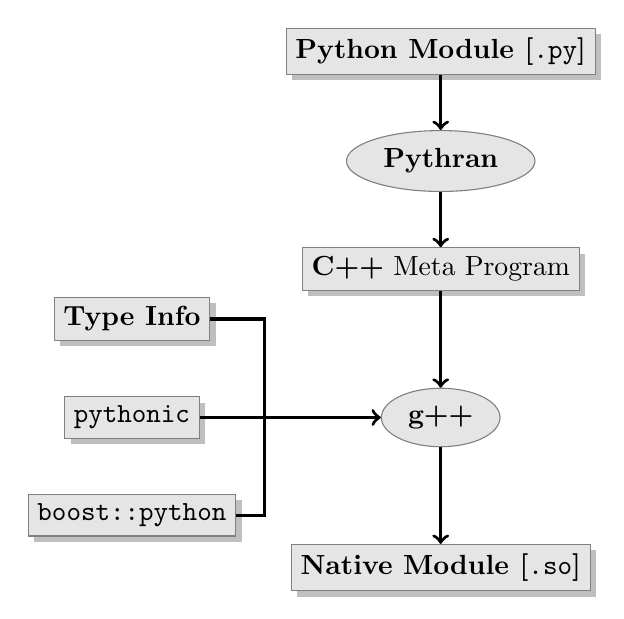
\begin{tikzpicture}[
            file/.style={draw=black!50,fill=black!10,rectangle, drop shadow, align=center,
            node distance=0.7cm},
            tool/.style={draw=black!50,fill=black!10,ellipse, align=center, node
        distance=0.7cm}]
        \node[file] (python) {\textbf{Python Module [\texttt{.py}]}};
        \node[tool] (pythran) [below=of python] {\textbf{Pythran}};
        \node[file] (meta-cxx) [below=of pythran] {\textbf{C++} Meta Program};
        \node[tool] (gxx) [yshift=-1.5em, below=of meta-cxx] {\textbf{g++}};
        \node (empty) [xshift=-1em, left=of gxx] {};
        \node[file] (pythonic) [left=of empty] {\textbf{\texttt{pythonic}}};
        \node[file] (annotation)     [above=of pythonic] {\textbf{Type Info}};
        \node[file] (boost) [below=of pythonic] {\textbf{\texttt{boost::python}}};
        \node[file] (so) [yshift=-1.5em, below=of gxx] {\textbf{Native Module [\texttt{.so}]}};

        \draw[very thick, ->] (python) -- (pythran);
        \draw[very thick] (annotation) -| (empty.center);
        \draw[very thick, ->] (pythran) -- (meta-cxx);
        \draw[very thick, ->] (meta-cxx) -- (gxx);
        \draw[very thick] (boost) -| (empty.center);
        \draw[very thick, ->] (pythonic) -- (gxx);
        \draw[very thick, ->] (gxx) -- (so);
    \end{tikzpicture}
    
    \caption{Pythran compilation flow.}
    \label{fig:pythran-compiler}

\end{figure}



\section{Code Analyses}
\label{sec:analysis}

A code analysis is a function that takes a part of the IR (or the whole
module's IR) as input and returns aggregated high-level information. For
instance, a simple Pythran analysis called \texttt{Identifiers} gathers the set
of all identifiers used throughout the program. This information is later used
when the creation of new identifiers is required so that no conflict occurs
with existing ones.

One of the most important analysis in Pythran is the \textbf{alias analysis}, sometimes
referred as \textbf{points-to} analysis. For each identifier, it computes an
approximation of the set of locations this identifier may points to. For
instance, let us consider the polymorphic function \texttt{foo} defined as follows:

\begin{lstlisting}
def foo(a,b):
    c = a or b
    return c * 2
\end{lstlisting}

The identifier \texttt{c} involved in the multiplication may refer to

\begin{itemize}
    \item a fresh location if \texttt{a} and \texttt{b} are scalars

    \item the same location as \texttt{a} if \texttt{a} evaluates to \texttt{True}

    \item the same location as \texttt{b} otherwise.

\end{itemize}

As we do not specialise the analysis for different types and the truth value of
\texttt{a} is unknown at compilation time, the alias analysis yields the approximated
result that \texttt{c} may point to a fresh location, \texttt{a} or \texttt{b}.

Without this kind of information, even a simple instruction like
\texttt{sum(a)} would yield very few informations as there is no guarantee that
the \texttt{sum} identifiers points to the \texttt{sum} built-in, as someone
could have previously stated that \texttt{sum = len}.

When turning Python AST to Pythran IR, nested functions are turned into global
functions taking their expanded closure as parameter. This closure is computed using the
information provided by the \texttt{Globals} analysis that statically computes the
state of the dictionary of globals, and \texttt{ImportedIds} that computes the set of
identifiers used by an instruction but not declared in this instruction. For
instance in the following snippet:

\begin{lstlisting}
def outer(outer_argument):
    def inner(inner_argument):
        return cos(outer_argument) + inner_argument
        return inner(3)
\end{lstlisting}

The \texttt{Globals} analysis called on the \texttt{inner} function definition
marks \texttt{cos} as a global variable, and \texttt{ImportedIds} marks
\texttt{outer\_argument} and \texttt{cos} as imported identifiers. The result
of the transformation of nested function into global functions on that
particular example is:

\begin{lstlisting}
import functools

def _inner(outer_argument, inner_argument):
    return cos(outer_argument) + inner_argument

def outer(outer_argument):
    inner = functools.partial(_inner, outer_argument)
    return inner(3)
\end{lstlisting}

A rather high-level analysis is the \texttt{PureFunctions} analysis, that computes the
set of functions declared in the module that are pure, i.e. whose return value
only depends from the value of their argument. This analysis depends on two
other analyses, namely \texttt{GlobalEffects} that computes for each function whether
this function modifies the global state (including I/O, random generators, etc.)
and \texttt{ArgumentEffects} that computes for each argument of each function whether
this argument may be updated in the function body. These three analyses work
inter-procedurally, as illustrated by the following example:

\begin{lstlisting}
def fibo(n):
    return n if n < 2 else fibo(n - 1) + fibo(n - 2)

def bar(l):
    return map(fibo, l)

def foo(l):
    return map(fibo, random.sample(l, 3))
\end{lstlisting}

The \texttt{fibo} function is pure as it has no global effects or argument effects and
only calls itself. As a consequence the \texttt{bar} function is also pure as the
\texttt{map} intrinsic is pure when its first argument is pure. However the \texttt{foo}
function is not pure as it calls the \texttt{sample} function from the \texttt{random}
module, which has a global effect (on the underlying random number generator
internal state).

Several analyses depend on the \texttt{PureFunctions} analysis.
\texttt{ParallelMaps} uses aliasing information to check if an identifier
points to the \texttt{map} intrinsic, and checks if the first argument is a
pure function using \texttt{PureFunctions}. In that case the \texttt{map} is
added to the set of parallel maps, because it can be executed in any order.
This is the case for the first \texttt{map} in the following snippet, but not
for the second because the \texttt{print b} involves an \textbf{I/O}.

\begin{lstlisting}
def pure(a):
    return a ** 2

def guilty(a):
    b = pure(a)
    print b
    return b

l = list(...)
map(pure, l)
map(guilty, l)
\end{lstlisting}

\texttt{ConstantExpressions} uses function purity to decide whether a given expression
is constant, i.e. its value only depends on literals. For instance the
expression \texttt{fibo(12)} is a constant expression because \texttt{fibo} is pure and its
argument is a literal.

\texttt{UseDefChains} is a classical analysis from the static compilation world. For
each variable defined in a function, it computes the chain of \textbf{use} and \textbf{def}.
The result can be used to drive various code transformations, for instance to
remove dead code, as a \textbf{def} followed by a \textbf{def} or nothing is useless. It is
used in Pythran to avoid false polymorphism. An intuitive way to represent
use-def chains is illustrated on next code snippet:

\begin{lstlisting}
a = 1
if cond:
    a = a + 2
else:
    a = 3
print a
a = 4
\end{lstlisting}

In this example, there are two possible chains starting from the first
assignment. Using \texttt{U} to denote \textbf{use} and \texttt{D} to denote \textbf{def}, one gets:

\begin{center}
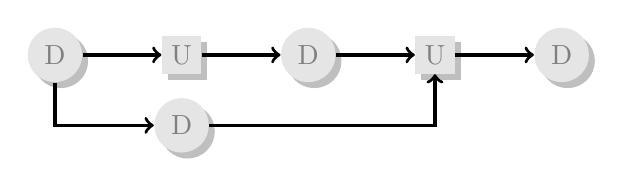
\begin{tikzpicture}[D/.style={black!50,fill=black!10, circle, drop shadow, align=center},
    U/.style={black!50,fill=black!10, rectangle, drop shadow, align=center}]
    \node[D] (d0) {D};
    \node[U] (u0) [right=of d0] {U};
    \node[D] (d1) [right=of u0] {D};
    \node[U] (u1) [right=of d1] {U};
    \node[D] (d2) [right=of u1] {D};

    \node[D] (dp0)[below=of u0, yshift=2em] {D};

    \draw[very thick, ->] (d0) -- (u0);
    \draw[very thick, ->] (d0) |- (dp0);
    \draw[very thick, ->] (u0) -- (d1);
    \draw[very thick, ->] (d1) -- (u1);
    \draw[very thick, ->] (dp0) -| (u1);
    \draw[very thick, ->] (u1) -- (d2);
\end{tikzpicture}
\end{center}

The fact that all paths finish by a \textbf{def} indicates that the last
assignment can be removed (but not necessarily its right hand part that could
have a side-effect). The fact that the last \textbf{use} is always preceded by
a \textbf{def}taht only point to it indicates that these \textbf{def}s can
safely be renamed from \texttt{a} to \texttt{a}' (thus performing scalar
renaming).

All the above analyses are used by the Pythran developer to build code
transformations that improve the execution time of the generated code.

\section{Code Optimizations}
\label{sec:optimizations}

One of the benefits of translating Python code to C++ code is that it removes
most of the dynamic lookups. It also unveils all the optimizations available at
C++ level. For instance, a function call is quite costly in Python, which
advocates in favor of using inlining. This transformation comes at no cost when
using C++ as the back-end language, as the C++ compiler does it.

However, there are some informations available at the Python level that cannot
be recovered at the C++ level. For instance, Pythran uses functor with an
internal state and a goto dispatch table to represent generators. Although
effective, this approach is not very efficient, especially for trivial cases.
Such trivial cases appear when a generator expression is converted, in the
front-end, to a looping generator. To avoid this extra cost, Pythran turns
generator expressions into call to \texttt{imap} and \texttt{ifilter} from the
\texttt{itertools} module whenever possible, removing the unnecessary goto
dispatching table. This kind of transformation cannot be made by the C++
compiler. For instance, the one-liner \texttt{len(set(vec[i]+i for i in cols))}
extracted from the \texttt{nqueens} benchmarks from the Unladen Swallow project
is rewritten as \texttt{len(set(itertools.imap(lambda i: vec[i]+i,cols)))}.
This new form is less efficient in pure Python (it implies one extra function
call per iteration), but can be compiled into C++ more efficiently than a
generic generator.

A similar optimization consists in turning \texttt{map}, \texttt{zip} or
\texttt{filter} into their equivalent version from the \texttt{itertool}
module. The benefit is twofold: first it removes a temporary allocation, second
it gives an opportunity to the compiler to replace list accesses by scalar
accesses. This transformation is not always valid, nor profitable. It is not
valid if the content of the output list is written later on, and not profitable
if the content of the output list is read several times, as each read implies
the (re) computation, as illustrated in the following code:

\begin{lstlisting}
def valid_conversion(n):
    # this map can be converted to imap
    l = map(math.cos, range(n))
    return sum(l) # sum iterates once on its input

def invalid_conversion(n):
    # this map cannot be converted to imap
    l = map(math.cos, range(n))
    l[0] = 1  # invalid assignment
    return sum(l) + max(l) # sum iterates once
\end{lstlisting}

The information concerning constant expressions is used to perform a classical
transformation called \texttt{ConstantFolding}, which consists in the compile-time
evaluation of constant expressions. The validity is guaranteed by the
\texttt{ConstantExpressions} analysis, and the evaluation relies on Python ability to
compile an AST into byte code and run it, benefiting from the fact that Pythran
IR is a subset of Python AST. A typical illustration is the initialization of a
cache at compile-time:

\begin{lstlisting}
def esieve(n):
    candidates = range(2, n+1)
    return sorted(
        set(candidates) - set(p*i
                              for p in candidates
                              for i in range(p, n+1))
        )

cache = esieve(100)
\end{lstlisting}

Pythran automatically detects that \texttt{eseive} is a pure function and evaluates
the \texttt{cache} variable value at compile time.

\texttt{ConstantFolding} may create a lot of candidates for \texttt{LoopUnrolling}. In Python, loops are used to iterate over sequences. If such a sequence is an explicit list, then Pythran unrolls the loop accordingly. Thanks to \texttt{ConstantFolding}, a call to \texttt{range(4)} will statically turn into \texttt{[0, 1, 2, 3]} (after a check that \texttt{range} actually points to \texttt{\_\_builtin\_\_.range}) making it possible to unroll the loop statically.

Sometimes, coders use the same variable in a function to represent value with
different types, which leads to false polymorphism, as in:


\begin{lstlisting}
a = cos(1)
a = str(a)
\end{lstlisting}

These instructions cannot be translated to C++ directly because \texttt{a}
would have both \texttt{double} and \texttt{str} type. However, using
\texttt{UseDefChains} it is possible to assert the validity of the renaming of
the instructions into:


\begin{lstlisting}
a = cos(1)
a_ = str(a)
\end{lstlisting}

that does not have the same typing issue.

In addition to these python-level optimizations, the Pythran back end library,
\texttt{pythonic}, uses several well known optimizations, especially for Numpy
expressions.

\section{Library Level Optimizations}
\label{sec:backend}

Using the proper library, the C++ language provides an abstraction level close
to what Python proposes. Pythran provides a wrapper library, \texttt{pythonic},
that leverage on the C++ Standard Template Library (STL), the GNU Multiple
Precision Arithmetic Library (GMP) and the Numerical Template Toolbox
(NT2)\footnote{\url{https://github.com/MetaScale/nt2}} to emulate Python
standard library. The STL is used to provide a typed version of the standard
containers (\texttt{list}, \texttt{set}, \texttt{dict} and \texttt{str}), as
well as reference-based memory management through \texttt{shared\_ptr}. Generic
algorithms such as \texttt{accumulate} are used when possible. GMP is the
natural pick to represent Python's \texttt{long} in C++. NT2 provides a generic
vector library called \texttt{boost.simd}\cite{esterie2012boost} that enables
the vector instruction units of modern processors in a generic way. It is used
to efficiently compile Numpy expressions.

Numpy expressions are the perfect candidates for library level optimizations.
Pythran implements three optimizations on such expressions:

\begin{enumerate}

    \item Expression templates\cite{expression_templates} are used to avoid
        multiple iterations and the creation of intermediate arrays. Because
        they aggregates all \texttt{ufunc} into a single expression at compile
        time, they also increase the computation intensity of the loop body,
        which increases the impact of the two following optimizations.

    \item Loop vectorization. All modern processors have vector instruction
        units capable of applying the same operation on a vector of data
        instead of a single data. For instance Intel Sandy Bridge can run 8
        single-precision additions per instruction. One can directly use the
        vector instruction set assembly to use these vector units, or use C/C++
        intrinsics. Pythran relies on \texttt{boost.simd} from NT2 that offers
        a generic vector implementation of all standard math functions to
        generate a vectorized version of Numpy expressions. Again, the
        aggregation of operators performed by the expression templates proves
        to be beneficial, as it reduces the number of (costly) loads from the
        main memory to the vector unit.

    \item Loop parallelization through OpenMP\cite{openmp3.1}. Numpy expression
        computation do not carry any loop-dependency. They are perfect
        candidates for loop parallelization, especially after the expression
        templates aggregation, as OpenMP generally performs better on loops
        with higher computation intensity that masks the scheduling overhead.

\end{enumerate}

To illustrate the benefits of these three optimizations combined, let us
consider the simple Numpy expression:

\begin{lstlisting}
d = numpy.sqrt(b*b+c*c)
\end{lstlisting}

When benchmarked with the \texttt{timeit} module on an hyper-threaded quad-core i7, the
pure Python execution yields:

\begin{lstlisting}
>>> %timeit np.sqrt(b*b+c*c)
1000 loops, best of 3: 1.23 ms per loop
\end{lstlisting}

\noindent then after Pythran processing and using expression templates:

\begin{lstlisting}
>>> %timeit my.pythranized(b,c)
1000 loops, best of 3: 621 us per loop
\end{lstlisting}

The speed-up is due to the fact that expression templates replace 4 temporary
array creations and 4 loops by a single allocation and a single loop.

Going a step further and vectorizing the generated loop yields an extra
performance boost:

\begin{lstlisting}
>>> %timeit my.pythranized(b,c)
1000 loops, best of 3: 418 us per loop
\end{lstlisting}

Although the AVX instruction set makes it possible to store 4 double precision
floats, one does not get a 4x speed up because of the (unaligned) memory transfers
to and from vector registers.

Finally, using both expression templates, vectorization and OpenMP:

\begin{lstlisting}
>>> %timeit my.pythranized(b,c)
1000 loops, best of 3: 105 us per loop
\end{lstlisting}

The 4 hyper-threaded cores give an extra performance boost. Unfortunately, the
load is not sufficient to get more than an average 4x speed up compared to the
vectorized version. In the end, Pythran generates a native module that performs
roughly 11 times faster than the original version.

As a reference, the \texttt{numexpr} module that performs JIT optimization of the
expression yields the following timing:

\begin{lstlisting}
>>> %timeit numexpr.evaluate("sqrt(b*b+c*c)")
1000 loops, best of 3: 395 us per loop
\end{lstlisting}

\noindent Pythran still performs almost four times faster.

\section{Explicit Parallelization}
\label{sec:openmp}

Many scientific applications can benefit from the parallel execution of their
kernels. As modern computers generally feature several processors and several
cores per processor, it is critical for the scientific application developer to
be able to take advantage of them.

As explained in the previous section, Pythran takes advantage of multiple cores
when compiling Numpy expressions. However, when possible, it is often more
profitable to parallelize the outermost loops rather than the inner loops
---the Numpy expressions--- because it avoids the synchronization barrier at
the end of each parallel section, and generally offers more computation
intensive computations.

The OpenMP standard\cite{openmp3.1} is a widely used solution for Fortran, C
and C++ to describe loop-based and task-based parallelism. It consists of a few
directives attached to the code, that describe parallel loops and parallel code
sections in a shared memory model.

Pythran makes this directives available at the Python level through string
instructions. The semantic is roughly similar to the original semantics,
assuming that all variables have function level scope.

The following listing gives a simple example of explicit loop-based
parallelism.  OpenMP 3.0 task-based parallelism form is also supported, the
interested reader may refer to~\cite{pyhpc2013} for more details.

\begin{lstlisting}
def pi_estimate(darts):
    hits = 0
    #omp parallel for reduction(+:hits)"
    for i in xrange(darts):
        x,y = random(), random()
        dist = sqrt(pow(x, 2) + pow(y, 2))
        if dist <= 1.0:
            hits += 1.0
    pi = 4 * (hits / DARTS)
    return pi
\end{lstlisting}

The loop is flagged as parallel, performing a reduction using the \texttt{+}
operator on the \texttt{hits} variable. Variables \texttt{x}, \texttt{y} and
\texttt{dist} are automatically made local by Pythran after a
\texttt{ScopeAnalysis}, and are thus marked as \texttt{private}, i.e. local to
a thread and not shared with other threads, by OpenMP.

Next section performs an in-depth comparison of Pythran with for Python
optimizers: Numba, PyPy, ShedSkin and numexpr.


\section{Benchmarks}
\label{sec:benchmarks}


All benchmarks presented in this section are ran on an hyper-threaded quad-core
i7, using examples shipped along Pythran sources, available at
https://github.com/serge-sans-paille/pythran in the \texttt{pythran/test/cases}
directory. The Pythran version used is the \texttt{HEAD} of the \texttt{scipy2013} branch,
ShedSkin 0.9.2, PyPy 2.0 compiled with the \texttt{-jit} flag, CPython 2.7.3, Cython
0.19.1 and Numexpr 2.0.1. All timings are made using the \texttt{timeit} module,
taking the best of all runs. All C++ codes are compiled with g++ 4.7.3, using
the tool default compiler option, generally \texttt{-O2} plus a few optimizing flags
depending on the target.

Cython is not considered in most benchmarks, because to get an efficient
binary, one needs to rewrite the original code, while all the considered tools
are running the very same Python code that remains compatible with CPython. The
experiment was only done to have a comparison with Numexpr.

Pystone is a Python translation of whetstone, a famous floating point number
benchmarks that dates back to Algol60 and the 70's. Although non representative
of real applications, it illustrates the general performance of floating point
number manipulations. Table \ref{tbl:pystone}  illustrates the benchmark
result for CPython, PyPy, ShedSkin and Pythran, using an input value of
\texttt{10**3}. Note that the original version has been updated to replace the user
class by a function call.

\begin{table}
    \centering

    \begin{tabular}{|l|c|c|c|c|}
        \hline
     Tool    &  CPython    &   Pythran     &     PyPy   &  ShedSkin  \\
    \hline
     Timing  &  861ms      &   11.8ms      &     29.1ms &  24.7ms    \\
    \hline
     Speedup &  $\times$1         &   $\times$72.9       &    $\times$29.6   &  $\times$34.8     \\
    \hline
\end{tabular}

    \caption{Benchmarking result on the Pystone program.}
    \label{tbl:pystone}

\end{table}

It comes at no surprise that all tools get more than decent results on this
benchmark. PyPy generates a code almost as efficient as ShedSkin. Altough both
generate C++, Pythran outperforms ShedSkin thanks to a higher level generated
code. For instance all arrays are represented in ShedSkin by pointers to arrays
that likely disturbs the g++ optimizer, while Pythran uses a vector class wrapping
shared pointers.

Nqueen is a benchmark extracted from the former Unladen Swallow\footnote{\url{http://code.google.com/p/unladen-swallow/}} project. It
is particularly interesting as it makes an intensive use of non-trivial
generator expressions and integer sets. Table\ref{tbl:nqueen} illustrates
the benchmark results for CPython, PyPy, ShedSkin and Pythran. The code had to
be slightly updated to run with ShedSkin because type inference in ShedSkin does
not support mixed scalar and \textbf{None} variables. The input value is \texttt{9}.

\begin{table}
    \centering

    \begin{tabular}{|l|c|c|c|c|}
        \hline
     Tool    &  CPython    &   Pythran     &     PyPy   &  ShedSkin \\
    \hline
     Timing  &  1904.6ms   &   358.3ms     &    546.1ms &  701.5ms  \\
    \hline
     Speedup &  $\times$1         &    $\times$5.31      &    $\times$3.49   &  $\times$2.71    \\
    \hline
\end{tabular}
\caption{Benchmarking result on the NQueen program.}
\label{tbl:nqueen}

\end{table}

It seems that compilers have difficulties to take advantage of high level
constructs such as generator expressions, as the overall speedup is not
breathtaking. Pythran benefits from the conversion to \texttt{itertools.imap} here,
while ShedSkin and PyPy rely on more costly constructs. A deeper look at the
Pythran profiling trace shows that more than half of the execution time is
spent allocating and deallocating a \texttt{set} used in the internal loop. There is a
memory allocation invariant that could be taken advantage of there, but none of
the compiler does.

Hyantes\footnote{\url{http://hyantes.gforge.inria.fr}} is a geomatic application that exhibits typical usage of arrays
using loops instead of generalized expressions. It is helpful to measure the
performance of direct array indexing.

Table\ref{tbl:hyantes} illustrates the benchmark result for CPython, PyPy,
ShedSkin and Pythran, when using lists as the data container. The output window
used is \texttt{100x100}.

\begin{table}
    \centering

    \begin{tabular}{|l|c|c|c|c|}

        \hline
     Tool    &  CPython    &   Pythran     &     PyPy   &  ShedSkin  \\
    \hline
     Timing  &  1295.4ms   &   270.5ms     &    277.5ms &  281.5ms   \\
    \hline
     Speedup &  x1         &    x4.79      &    x4.67   &  x4.60     \\
    \hline
\end{tabular}
\caption{Benchmarking result on the hyantes kernel, list version.}
\label{tbl:hyantes}

\end{table}

The speed ups are not amazing for a numerical application. there are two
reasons for this poor speedups. First, the \texttt{hyantes} benchmark makes heavy
usage of trigonometric functions, and there is not much gain there. Second, and
most important, the benchmark produces a big 2D array stored as a list of list,
so the application suffers from the heavy overhead of converting them from C++
to Python. Running the same benchmark using Numpy arrays as core containers
confirms this assumption, as illustrated by Table \ref{tbl:np-hyantes}. This
table also demonstrates the benefits of manual parallelization using OpenMP.


\begin{table}
    \centering

    \begin{tabular}{|l|c|c|c|c|}

        \hline
     Tool    &  CPython    &   Pythran     & Pythran+OpenMP   \\
    \hline
     Timing  &  450.0ms    &   4.8ms       &      2.3ms       \\
    \hline
     Speedup &  x1         &    x93.8      &    x195.7        \\
    \hline
\end{tabular}
\caption{Benchmarking result on the hyantes kernel, numpy version.}
\label{tbl:np-hyantes}
\end{table}

Finally, \texttt{arc\_distance} \footnote{The \texttt{arc\_distance} testbed is taken from to \url{https://bitbucket.org/FedericoV/numpy-tip-complex-modeling}.} presents a classical usage of Numpy expression. It
is typically more efficient than its loop alternative as all the iterations are
done directly in C. Its code is reproduced below:

\begin{lstlisting}
def arc_distance(theta_1, phi_1, theta_2, phi_2):
    """
    Calculates the pairwise arc distance
    between all points in vector a and b.
    """
    temp = (np.sin((theta_2-theta_1)/2)**2
        + np.cos(theta_1)*np.cos(theta_2)
          * np.sin((phi_2-phi_1)/2)**2)
    distance_matrix = 2 * np.arctan2(
            sqrt(temp),sqrt(1-temp))
    return distance_matrix
\end{lstlisting}


Table \ref{tbl:arc-distance} illustrates the benchmark result for CPython,
Cython, Numexpr and Pythran, using random input arrays of \texttt{10**6} elements.
Table \ref{tbl:arc-distance-2} details the Pythran performance. Cython code
is written using the \texttt{parallel.prange} feature and compiled with
\texttt{-fopenmp -O2 -march=native}.


\begin{table}
    \centering
    \begin{tabular}{|l|c|c|c|c|}
    \hline
     Tool    &  CPython    &  Cython  &  Numexpr    & Pythran   \\
    \hline
     Timing  &  192.2ms    &  36.0ms  &    41.2ms   &  17.1ms   \\
    \hline
     Speedup &  x1         &  x5.33   &  x4.67      &  x11.23   \\
    \hline
\end{tabular}
\caption{Benchmarking result on the arc distance kernel.}
\label{tbl:arc-distance}
\end{table}

\begin{table}
    \centering
    \begin{tabular}{|l|c|c|c|c|}
    \hline
    Tool & Pythran (raw) & Pythran (+AVX) & Pythran (+OMP) & Pythran (full)  \\
    \hline
    Timing & 186.3ms     &    75.4ms      &    41.1ms      &  17.1ms         \\
    \hline
    Speedup&    x1.03      &    x2.54       &    x4.67       &  x11.23         \\
    \hline
\end{tabular}
\caption{Benchmarking result on the arc distance kernel, Pythran details.}
\label{tbl:arc-distance-2}
\end{table}

It shows a small benefit from using expression templates on their own, most
certainly because the loop control overhead is negligible in front of the
trigonometric functions. It gets a decent x2.5 speed-up when using AVX over not
using it. The benefit of OpenMP, although related to the number of cores, makes
a whole speedup greater than x11 over the original Numpy version, without
changing the input code. Quite the opposite, Numexpr requires rewriting the input
and does not achieve the same level of performance as Pythran when OpenMP and
AVX are combined.

Writing efficient Cython code requires more work than just typing the variable
declarations using Cython's specific syntax: it only takes advantage of
parallelism because we made it explicit. Without explicit parallelization,
the generated code runs around 176ms instead of 36ms. Cython does not generate
vectorized code, and \texttt{gcc} does not vectorize the inner loop, which explains
the better result obtained with Pythran.

\section{Future Work}

Although Pythran focuses on a subset of Python and its standard library, many
optimizations opportunities are still possible. Using as Domain Specific
Language(DSL) approach, one could use rewriting rules to optimize several
Python idioms. For instance, \texttt{len(set(x))} could lead to an optimized
\texttt{count\_uniq} that would iterate only once on the input sequence.

There is naturally more work to be done at the Numpy level, for instance to
support more functions from the original module. The extraction of Numpy
expressions from \texttt{for loops} is also a natural optimization candidate, which
shares similarities with code refactoring.

Numpy expressions also fit perfectly well in the polyhedral model. Exploring
the coupling of polyhedral tools with the code generated from Pythran offers
enthusiastic perspectives.

\section{Conclusion}

This paper presents the Pythran compiler, a translator, and an optimizer, that
converts Python to C++. Unlike existing static compilers for Python, Pythran
leverages several function-level or module-level analyses to provide several
generic or Python-centric code optimizations. Additionally, it uses a C++
library that makes heavy usage of template programming to provide an efficient
API similar to a subset of Python standard library. This library takes
advantage of modern hardware capabilities ---vector instruction units and
multi-cores--- in its implementation of parts of the \texttt{numpy} package.

This paper gives an overview of the compilation flow, the analyses involved and
the optimizations used. It also compares the performance of compiled Pythran
modules against CPython and other optimizers: ShedSkin, PyPy and numexpr.

To conclude, limiting Python to a statically typed subset does not hinders the
expressivity when it comes to scientific or mathematic computations, but makes
it possible to use a wide variety of classical optimizations to help Python
match the performance of statically compiled language. Moreover, one can use
high level information to generate efficient code that would be difficult to write for the average programmer.

\acks

This project has been partially funded by the CARP Project and the SILKAN
Company.

% We recommend abbrvnat bibliography style.

\bibliographystyle{abbrvnat}
\bibliography{biblio}


\end{document}
